\subsection{UC2 - Visualizzazione indice della qualità delle previsioni}
\begin{figure}[H]
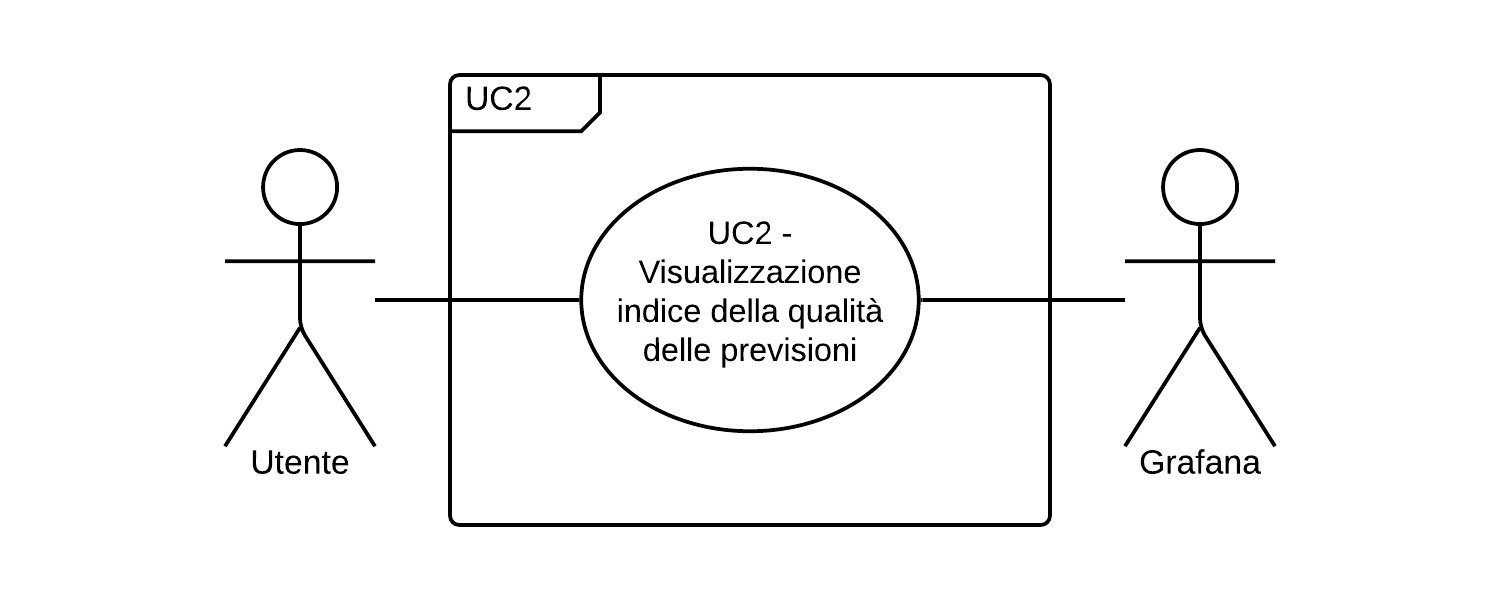
\includegraphics{img/UC2_-_Visualizzazione_indice_della_qualit_delle_previsioni.png}
\caption{Diagramma degli use case di UC2}
\end{figure}
\begin{itemize}
	\item \textbf{Codice identificativo}: UC2;
	\item \textbf{Titolo}: visualizzazione indice della qualità delle previsioni;
	\item \textbf{Attori primari}: utente;
	\item \textbf{Attori secondari}: Grafana\glo;
	\item \textbf{Descrizione}: l'utente visualizza l'indice della qualità delle previsioni eseguite sui dati forniti;
	\item \textbf{Precondizioni}: l'utente ha eseguito l'addestramento interno a Grafana\glo;
	\item \textbf{Postcondizioni}: l'utente ha visualizzato l'indice della qualità delle previsioni;
	\item \textbf{Scenario principale}: l'utente visualizza l'indice della qualità delle previsioni.
\end{itemize}